\section{Preliminaries}\label{s:preliminaries}

\begin{figure*}[t]
\def\bb{\rule{2in}{0pt}\rule{0pt}{1in}}
\begin{center}
% \includegraphics[width=\linewidth,trim=0 170 70 0,clip ]{method/overview_v3.pdf}
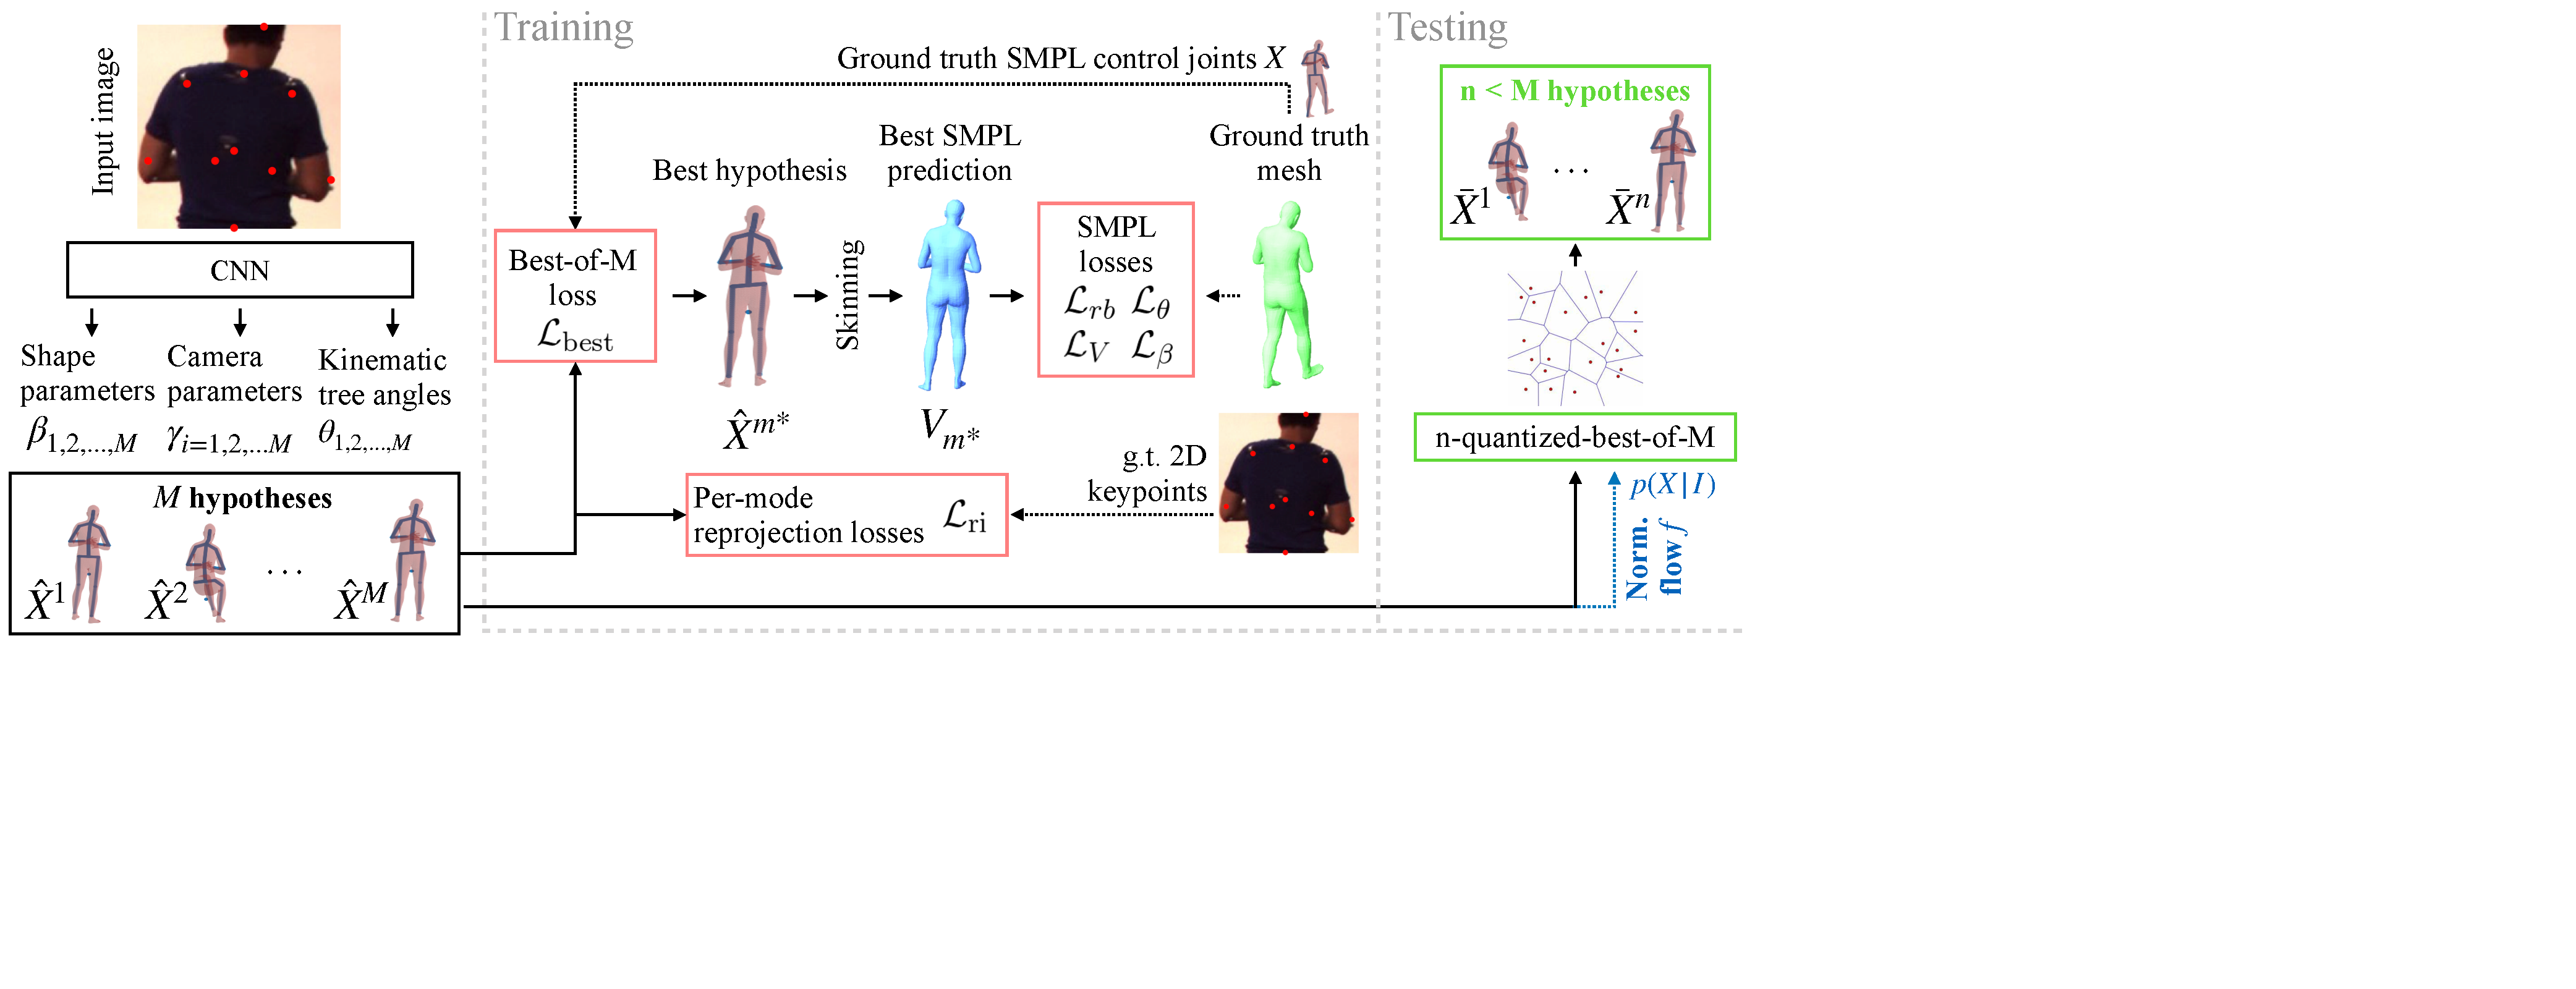
\includegraphics[width=\linewidth]{method/overview_v6.pdf}
\end{center}
\caption{\textbf{Overview of our method.}
Given a single image of a human, during training, our method produces multiple skeleton hypotheses $\{\hat X^i\}_{i=1}^M$ that enter a Best-of-$M$ loss which selects the representative $\hat X^{m^*}$ which most accurately matches the ground truth control joints $X$. 
% The camera parameters together with a skinned SMPL mesh enter the final set of SMPL losses.
At test time, we sample an arbitrary number of $n<M$ hypotheses by quantizing the set $\{\hat X^i\}$ that is assumed to be sampled from the probability distribution $p(X|I)$ modeled with normalizing flow $f$.
}\label{fig:arch_diagram}
\end{figure*}

Before discussing our method, we describe the necessary background, starting from SMPL\@.

\subsection{SMPL.}

SMPL is a model of the human body parameterized by axis-angle rotations $\theta \in \mathbb{R}^{69}$ of 23 body joints, the shape coefficients $\beta \in \mathbb{R}^{10}$ modelling shape variations, and a global rotation $\gamma \in \mathbb{R}^{3}$.
SMPL defines a \emph{skinning function}  $S: (\theta, \beta, \gamma) \mapsto V$ that maps the body parameters to the vertices $V \in \mathbb{R}^{6890\times 3}$ of a 3D mesh.
% The skinngin n itself is non-linear due to the conversion of the rotation angles into rotation matrices when the kinematic tree is assembled.

\subsection{Predicting the SMPL parameters from a single image.}

Given an image $\mathbf{I}$ containing a person, the goal is to recover the SMPL parameters $(\theta, \beta, \gamma)$ that provide the best 3D reconstruction of it.
% Conceptually, this is an inverse problem since the image $\mathbf{I} = \Gamma(S(\theta, \beta, \gamma), \eta)$ can be thought to be generated from the SMPL parameters $(\theta, \beta, \gamma)$ plus a number of unknown factors $\eta$ capturing details of the appearance, background, etc.
Existing algorithms~\cite{kanazawa18learning} cast this as learning a deep network $G(I) = (\theta, \beta, \gamma, t)$ that predicts the SMPL parameters as well as the %scale $s \in \mathbb{R}$ and
translation $t \in \mathbb{R}^3$ of the perspective camera observing the person. We assume a fixed set of camera parameters.
% \rk{TODO: Ben refines: The camera defines a function $\pi_{s,t}(X) = sx + t_{x}, sy + t_{y}$ projecting 3D points $X\in\mathbb{R}^3$ to 2D image coordinates: https://github.com/nkolot/SPIN/blob/b95a00a7c0147f2c5bee0874ba0972c6389b6f99/demo.py}.
During training, the camera is used to constrain the reconstructed 3D mesh and the annotated 2D keypoints to be consistent.
Since most datasets only contain annotations for a small set of keypoints (\cite{guler2018densepose} is an exception), and since these keypoints do not correspond directly to any of the SMPL mesh vertices, we need a mechanism to translate between them.
This mechanism is a fixed linear regressor $J : V \mapsto X$ that maps the SMPL mesh vertices $V = S(G(I))$ to the 3D locations $X = J(V) = J(S(G(I)))$ of the $K$ joints.
Then, the projections $\pi_{t}(X)$ of the 3D joint positions into image $\mathbf{I}$ can be compared to the available 2D annotations.

\subsection{Normalizing flows.}

The idea of normalizing flows (NF) is to represent a complex distribution $p(X)$ on a random variable $X$ as a much simpler distribution $p(z)$ on a transformed version $z=f(X)$ of $X$.
The transformation $f$ is learned so that $p(z)$ has a fixed shape, usually a Normal $p(z) \sim \mathcal{N}(0,1)$. Furthermore, $f$ itself must be \emph{invertible} and \emph{smooth}.
In this paper, we utilize a particular version of NF dubbed RealNVP \cite{dinh17density}.
A more detailed explanation of NF and RealNVP has been deferred to the supplementary.

% The idea of normalizing flows is to represent a complex distribution $p(X)$ on a random variable $X$ as a much simpler distribution $p(z)$ on a transformed version $z=f(X)$ of $X$.
% The transformation $f$ is learned so that $p(z)$ has a fixed shape, usually a Normal $p(z) \sim \mathcal{N}(0,1)$.
% Furthermore, $f$ itself must be \emph{invertible} and \emph{smooth}.
% In this case, the relation between $p(\theta)$ and $p(z)$ is given by a change of variable
% $$
%  p(z = f(X)) =  \left| \frac{df(X)}{dX} \right| p(X),
% $$
% where, for notational simplicity, we have assumed that $z,X\in\mathbb{R}^D$ are vectors.

% The challenge is to learn $f$ from data in a way that maintains its invertibility and smoothness.
% This is done by decomposing $z = f_L \circ \dots \circ f_1 (X)$ in $n$ layers, where $X_l = f_l(X_{l-1})$, $x = X_n$ and $X=X_0$, and each layer is in turn smooth and invertible.
% Then one can write
% $$
%  \log p(z = f(X)) =
%  \log p(X) + \sum_{l=1}^L \log \left| \frac{df_l(X_{l-1})}{dX_{l-1}} \right|.
% $$
% Now the challenge reduces to making sure that individual layers are in fact smooth and invertible and that their inverses and Jacobian determinants are easy to compute.
% RealNVP~\cite{dinh17density} does so by writing each layer as $f_l(X_{0:d,l}, X_{d:D,l-1}) = \big(X_{0:d,l-1},~ X_{d:D,l-1} \odot e^{g_l(X_{0:d,l-1})} + h_i(X_{0:d,l-1})\big)$ where $g_l,h_l:\mathbb{R}^d \rightarrow \mathbb{R}^{D-d}$ are two arbitrary neural networks.

\subsection{Method}\label{s:method}

% \subsection{Predicting multiple hypotheses.}

We start from a neural network architecture that implements the function  $G(I) = (\theta, \beta, \gamma, t)$ described above.
As shown in SPIN \cite{kolotouros19learning}, the HMR \cite{kanazawa18learning} architecture attains state-of-the-art results for this task, so we use it here.
However, the resulting regressor $G(I)$, given an input image $I$, can only produce a single unique solution.
In general, and in particular for cases with a high degree of reconstruction ambiguity, we are interested in predicting  \emph{set} of plausible 3D poses rather than a single one.
%
We thus extend our model to explicitly produce a set of $M$ different hypotheses $G_m (I) = (\theta_m, \beta_m, \gamma_m, t_m)$, $m=1,\dots,M$.
This is easily achieved by modifying the HMR's final output layer to produce a tensor $M$ times larger, effectively stacking the hypotheses.
In what follows, we describe the learning scheme that drives the monocular predictor $G$ to achieve
% uniform and precise coverage of all plausible poses consistent with the input image.
an optimal coverage of the plausible poses consistent with the input image. Our method is summarized in~\cref{fig:arch_diagram}. 

\subsection{Learning with multiple hypotheses}

For learning the model, we assume to have a training set of $N$ images $\{I_i\}_{i =1,\dots,N}$, each cropped around a person.
Furthermore, for each training image $I_i$ we assume to know (1) the 2D location $Y_i$ of the body joints (2) their 3D location $X_i$, and (3) the ground truth SMPL fit $(\theta_i, \beta_i, \gamma_i)$.
Depending on the set up, some of these quantities can be inferred from the others (e.g.~we can use the function $J$ to convert the SMPL parameters to the 3D joints $X_i$ and then the camera projection to obtain $Y_i$).

\subsection{Best-of-$M$ loss.}
Given a single input image, our network predicts a set of poses, where at least one should be similar to the ground truth annotation $X_i$.
This is captured by the best-of-$M$ loss~\cite{guzman2012multiple}:
\begin{equation}\label{e:loss-best}
  \mathcal{L}_\text{best}(J,G;m^*)
  =
  \frac{1}{N}
  \sum_{i=1}^N
  \big \| X_i - \hat X^{m_i^*}(I_i) \big \|,
  ~~
  m_i^*
  =
  \operatornamewithlimits{argmin}_{m=1,\dots,M}
  \big \| X_i -  \hat X^{m}(I_i) \big \|,
\end{equation}
where $\hat X^{m}(I_i) = J(G_m(V(I_i)))$ are the 3D joints estimated by the $m$-th SMPL predictor $G_m(I_i)$ applied to image $I_i$.
In this way, only the best hypothesis is steered to match the ground truth, leaving the other hypotheses free to sample the space of ambiguous solutions.
During the computation of this loss, we also extract the best index $m^*_i$ for each training example.

\subsection{Limitations of best-of-$M$.}

As noted in~\cref{s:intro}, best-of-$M$ only guarantees that one of the $M$ hypotheses is a good solution, but says nothing about the other ones.
Furthermore, in applications we are often interested in modulating the number of hypotheses generated, but the best-of-$M$ regressor $G(I)$ only produces a fixed number of output hypothesis $M$, and changing $M$ would require retraining from scratch, which is intractable.
% , in the sense that $G$ does not straightforwardly allow for outputting a different number of $n \neq M$ hypotheses.
% If a different number of hypotheses $M$ is desired, the na\:{\i}ve solution entails the intractably costly process of re-training $G$ for each possible value of $M$.
% If one wanted to output a different number of hypotheses, the na\"ive approach would entail the intractably costly process of re-training $G$ for each possible value of $M$.

We first address these issues by introducing a method that allows us to train a best-of-$M$ model for a large $M$ once and leverage it later to generate an arbitrary number of $n < M$ hypotheses without the need of retraining, while ensuring that these are good representatives of likely body poses.

\subsection{$n$-quantized-best-of-$M$}
Formally, given a set of $M$ predictions
$\mathcal{\hat X}^M(I) = \{\hat X^1(I), ..., \hat X^M(I)\}$ we seek to generate a smaller $n$-sized set
$\mathcal{\bar X}^n(I) = \{\bar X^1(I), ..., \bar X^n(I)\}$ which preserves the information contained in $\mathcal{\hat X}^M$.
In other words, $\mathcal{\bar X}^n$ \emph{optimally quantizes} $\mathcal{\hat X}^M$.
% To this end, inspired by the quantization literature \cite{gray1998quantization}, we define the best-of-$M$ quantization energy $E$ as:
% \begin{equation}\label{e:loss-quant}
% E(\mathcal{\hat X} | \mathcal{\bar X}) = \mathbb{E}_{p(\mathcal{\bar X})}
% \left[
%     \min_{\{\bar X^1, ... \bar X^n\}} \| \hat X^i - \bar X^j \|^2
% \right],
% \end{equation}
%
% \paragraph{$n$-quantized-best-of-$M$}
To this end, we interpret the output of the best-of-$M$ model as a set of choices $\mathcal{\hat X}^M(I)$ for the possible pose.
These poses are of course not all equally likely, but it is difficult to infer their probability from~\eqref{e:loss-best}.
We thus work with the following approximation.
We consider the prior $p(X)$ on possible poses (defined in the next section), and set:
\begin{equation}\label{e:conditional}
p(X|I)
=
p(X|\mathcal{\hat X}^M(I))
=
\sum_{i=1}^{M}
\delta({X} - \hat{X}^i(I))
\frac{p(\hat{X}^i(I))}{
\sum_{k=1}^{M} p(\hat{X}^k(I))}.
\end{equation}
This amounts to using the best-of-$M$ output as a conditioning \emph{set} (i.e.~an unweighted selection of plausible poses) and then use the prior $p(x)$ to weight the samples in this set.
With the weighted samples, we can then run $K$-means \cite{lloyd1982least} to further quantize the best-of-$M$ output while minimizing the quantization energy $E$:
\begin{equation}\label{e:loss-quant}
E(\mathcal{\bar X} | \mathcal{\hat X}) = \mathbb{E}_{p(X|I)}
\left[
    \min_{\{\bar X^1, ..., \bar X^n\}} \| X - \bar X^j \|^2
\right]
=
\sum_{i=1}^{M}
\frac{p(\hat{X}^i(I))}{
\sum_{k=1}^{M} p(\hat{X}^k(I))}
\min_{\{\bar X^1,\dots,\bar X^n\}}
\| \hat X^i(I) - \bar X^j \|^2.
\end{equation}
This can be done efficiently on GPU --- for our problem, K-Means consumes less than 20\% of the execution time of the entire forward pass of our method. 
% \rk{TODO: add in the Mean0 strategy to technical details.}

% Notice that, apart from the data vectors $\hat X$ and the quants $\bar X$, the quantization energy also assumes knowledge the probability density $p(\mathcal{\hat X})$ over the space of 3D skeletons $\mathcal{\hat X}$. \rk{justify that using prior $p(\mathcal{X})$ over the restricted set $\mathcal{\bar X}$ is in fact $p(\mathcal{X}|I)$}

\subsection{Learning the pose prior with normalizing flows.}
% In order to obtain $p(X)$, we propose to learn a deep generative model.
% While recent advances in generative modelling brought various possibilities (VAE \cite{}, GANs \cite{}), we opt for deep normalizing flows \cite{} due their intriguing property of being able to exactly maximize the data log likelihood.
In order to obtain $p(X)$, we propose to learn a normalizing flow model in form of
the RealNVP network $f$ described in \cref{s:preliminaries} and the supplementary. RealNVP optimizes the log likelihood $\mathcal{L}_\text{nf}(f)$ of training ground truth 3D skeletons $\{X_1, ... X_N\}$ annotated in their corresponding images $\{I_1, ..., I_N\}$ :
\begin{equation}\label{e:loglik}
\mathcal{L}_\text{nf}(f)
=
-
\frac{1}{N}
\sum_{i=1}^N
\log p(X_i)
=\\
-
\frac{1}{N}
\sum_{i=1}^N
\left(
\log \mathcal{N}(f(X_i))
-
\sum_{l=1}^L
\log
\left|
\frac{d f_l(X_{li})}{d X_{li}}
\right|
\right).
\end{equation}

\subsection{2D re-projection loss.}

Since the best-of-$M$ loss optimizes a single prediction at a time, often some members of the ensemble $\mathcal{\hat X}(I)$ drift away from the manifold of plausible human body shapes, ultimately becoming `dead' predictions that are never selected as the best hypothesis $m^*$.
In order to prevent this, we further utilize a re-projection loss that acts across all hypotheses for a given image.
More specifically, we constrain the set of 3D reconstructions to lie on projection rays passing through the 2D input keypoints with the following \emph{hypothesis re-projection loss}:
\begin{equation}\label{e:loss-ri}
  \mathcal{L}_\text{ri}(J,G)
  =
  \frac{1}{N}
  \sum_{i=1}^N
  \sum_{m=1}^M
  \big \| Y_i - \pi_{t_{i}}(\hat X^m(I)) \big \|.
\end{equation}

Note that many of our training images exhibit significant occlusion, so $Y$ may contain invisible or missing points. We handle this by masking $\mathcal{L}_\text{ri}$ to prevent these points contributing to the loss.

\paragraph{SMPL loss.}
The final loss terms, introduced by prior work~\cite{kanazawa18learning,pavlakos18learning,kolotouros19learning}, penalize
deviations between the predicted and ground truth SMPL parameters.
For our method, these are only applied to the best hypothesis $m_i^*$ found above:
% {\small
% \begin{align}\label{e:smpl}
% \mathcal{L}_\theta(G;m^*) =& \frac{1}{N}
%   \sum_{i=1}^N \| \theta_i - G_{\theta,m_i^*}(I_i)\| \\
% \mathcal{L}_\beta(G;m^*) =& \frac{1}{N} \label{e:smpl2}
%   \sum_{i=1}^N \| \beta_i - G_{\beta,m_i^*}(I_i)\| \\
% \mathcal{L}_V(G;m^*) =& \frac{1}{N} \label{e:smpl3}
%   \sum_{i=1}^N \| S(\theta_i,\beta_i,\gamma_i) - S(G_{(\theta,\beta,\gamma),m_i^*}(I_i))\| \\
% \mathcal{L}_\text{rb}(G;m^*) =& \frac{1}{N} \label{e:smpl4}
%   \sum_{i=1}^N \| \hat Y_i - \pi(s_{i}, t_{i})(\hat{X}^{m_i^*}(I_i))\|
% \end{align}
% }
{\small
\begin{align}
\mathcal{L}_\theta(G;m^*) = \frac{1}{N}
  \sum_{i=1}^N \| \theta_i - G_{\theta,m_i^*}(I_i)\|; &~
\mathcal{L}_V(G;m^*) = \frac{1}{N} \label{e:smpl}
  \sum_{i=1}^N \| S(\theta_i,\beta_i,\gamma_i) - S(G_{(\theta,\beta,\gamma),m_i^*}(I_i))\| \\
\mathcal{L}_\beta(G;m^*) = \frac{1}{N}
  \sum_{i=1}^N \| \beta_i - G_{\beta,m_i^*}(I_i)\|; &~
\mathcal{L}_\text{rb}(G;m^*) = \frac{1}{N} \label{e:smpl2}
  \sum_{i=1}^N \| Y_i - \pi_{t_{i}}(\hat{X}^{m_i^*}(I_i))\|
\end{align}}%
Note here we use $\mathcal{L}_\text{rb}$ to refer to a 2D re-projection error between the best hypothesis and ground truth 2D points $Y_i$. This differs from the earlier loss $\mathcal{L}_\text{ri}$, which is applied across all modes to enforce consistency to the visible \emph{input} points. Note that we could have used \cref{e:smpl,e:smpl2} to select the best hypothesis $m_i^*$, but it would entail an unmanageable memory footprint due to the requirement of SMPL-meshing for every hypothesis before the best-of-$M$ selection.


\subsection{Overall loss.}

The model is thus trained to minimize:
\begin{equation}\label{e:loss-total}
%   \begin{aligned}
%     \mathcal{L}(J,G)&=
%     \lambda_\text{nf} \mathcal{L}_\text{nf}(J,G) +
%     \lambda_\text{ri} \mathcal{L}_\text{ri}(J,G) \\& +
%     \lambda_\text{best} \mathcal{L}_\text{best}(J,G;m^*) +
%     \lambda_\theta \mathcal{L}_\theta(J,G;m^*) \\& +
%     \lambda_\beta \mathcal{L}_\beta(J,G;m^*) +
%     \lambda_\text{V} \mathcal{L}_V(J,G;m^*) \\& +
%     \lambda_\text{rb} \mathcal{L}_\text{rb}(J,G;m^*)
%   \end{aligned}
  \begin{aligned}
    \mathcal{L}(J,G)&=
    \lambda_\text{ri} \mathcal{L}_\text{ri}(J,G) +
    \lambda_\text{best} \mathcal{L}_\text{best}(J,G;m^*) +
    \lambda_\theta \mathcal{L}_\theta(J,G;m^*) \\& +
    \lambda_\beta \mathcal{L}_\beta(J,G;m^*) +
    \lambda_\text{V} \mathcal{L}_V(J,G;m^*) +
    \lambda_\text{rb} \mathcal{L}_\text{rb}(J,G;m^*)
  \end{aligned}
\end{equation}
where $m^*$ is given in~\cref{e:loss-best} and
$
\lambda_\text{ri},
\lambda_\text{best},
\lambda_\theta,
\lambda_\beta,
\lambda_\text{V},
\lambda_\text{rb}
$
are weighing factors.
We use a consistent set of SMPL loss weights across all experiments
$\lambda_\text{best}= 25.0, \lambda_\theta=1.0,
\lambda_\beta=0.001,
\lambda_\text{V}=1.0,
$ and set $\lambda_\text{ri} = 1.0$.
%
Since the training of the normalizing flow $f$ is independent of the rest of the model, we train $f$ separately by optimizing $\mathcal{L}_\text{nf}$ with the weight of $\lambda_\text{nf}=1.0$. Samples from our trained normalizing flow are shown in \cref{fig:nf_samples}

% place holder
% \begin{figure*}
%     \centering
%     \fbox{\makebox(460,100){}}
%     \caption{Best in blue, GT right most. \label{fig:h36m_qual}}
% \end{figure*}
% \newcommand{\vspacekill}{\vspace{-0.4cm}}
\newcommand{\flowfig}[1]{
\includegraphics[width=0.1\linewidth,trim=200 200 200 200,clip]{exps/flow_samples/sample_#1.png}}
% final figure
\begin{figure*}
    \centering
    \flowfig{00004}%
    \flowfig{00016}%
    \flowfig{00031}%
    \flowfig{00038}%
    \flowfig{00041}%
    \flowfig{00050}%
    \flowfig{00054}%
    \flowfig{00061}%
    \flowfig{00078}%
    \caption{%
    \textbf{Example samples from the normalizing flow} 
    $f: X \mapsto z;~ p(z) \sim \mathcal{N}(0,1)$,
    trained on a dataset of ground truth 3D SMPL control skeletons $\{X_1, ..., X_N\}$.
    }\label{fig:nf_samples}
\end{figure*}